\documentclass[12 pt, twoside]{article}

\usepackage[english]{babel}
\usepackage[letterpaper]{geometry}
\geometry{top = 1.0 in, bottom = 1.0 in, left = 1.0 in, right = 1.0 in}

\usepackage{graphicx}
\usepackage{float}
\usepackage{listings}
\usepackage{indentfirst}
\usepackage{mathtools}
\usepackage{amsmath}
\usepackage{enumerate}
\usepackage{subcaption}
\usepackage{units}
\usepackage{cases}
\usepackage{array}
\usepackage{multirow}

\begin{document}
	\begin{titlepage}		
		\begin{center}
			
\includegraphics[width = 6.0 in]{FIU_Logo.jpg} \\[0.2 in]
			
			\Large
			{
				College of Engineering and Computing \\[0.05 in]
				Department of Electrical and Computer Engineering \\[0.5 in]
			}
			
			
\includegraphics[width = 5.0 in]{UVA_Logo} \\[0.1 in]
			
			\Large
			{
				Institute for Informatics \\[0.05 in]
				SNE (Systems and Network Engineering Group) \\[0.5 in]
			}
			
			\textnormal{\Huge GEMBus Installation and Setup Log:} \\[0.4 in]
			
			\Large
			{
				\noindent NAME: \\
				Pedro D Bello-Maldonado \\[0.2 in]
				MENTORS: \\
				Dr. Paola Grosso \\
				Dr. Ana Oprescu \\[0.4 in]
				Summer 2013 
			}
		\end{center}
	\end{titlepage}
	
	\section{Introduction}
	{
		The purpose of this document is to expose some of the issues encountered while trying to enable all the GEMBus services. Some of these issues were resolved and will be explained here, and others were not. 
	}
	
	\section{GEMBus Services}
	{
		\subsection{The Registry Service:}
		{
			Following the instructions provided in \textbf{GEMBus cookbook}, I started by implementing the registry service. The registry folder contains a file called INSTALL that provides instructions of the packages necessary to use the service. Once these packages were installed, the setup.py program was executed as instructed but some packages were missing. To resolve this, I followed the instruction given in \textbf{Problems-with-cookbook} and I run the setup program again successfully.  \\
			
			After the installation went through, I proceeded to execute \textbf{app\_np.py} which starts the service according to the documentation. Doing this, however, threw errors stating that packages imported in the source code were missing. The modules and the sources that import them are listed next:
			
			\begin{itemize}
				\item \textbf{FILE:} http\_util.py \\
				\textbf{PATH:} /usr/local/lib/python2.7/dist-packages/registry-0.3.0-py2.7.egg/ \\ gembus/http\_util.py \\
				\textbf{ERROR:} No module named oic.utils
				\item \textbf{FILE:} organization.py \\
				\textbf{PATH:} /usr/local/lib/python2.7/dist-packages/registry-0.3.0-py2.7.egg/ \\ gembus/db/organization.py \\
				\textbf{ERROR:} No module named offer
			\end{itemize}
			
			After looking everywhere and not finding the missing packages I proceeded to comment the lines of code that imported these packages and run the application again with success. We tested the URL \textit{http://localhost:8087} were the service should be running at and it was working fine.
		}
		
		\subsection{The Repository Service:}
		{
			Installing the packages suggested in both the cookbook and Problems-with-cookbook led to a working service. This is what I got after adding the URL using \textbf{obr:addurl} and using the \textbf{deploy} command to deploy either \textbf{perfsonarNMWGAdapter} or \textbf{perfsonarRRDMAAdapter}. This information is find using \textbf{log:display}: \\
			
			\begin{figure}[!ht]
				\centering
				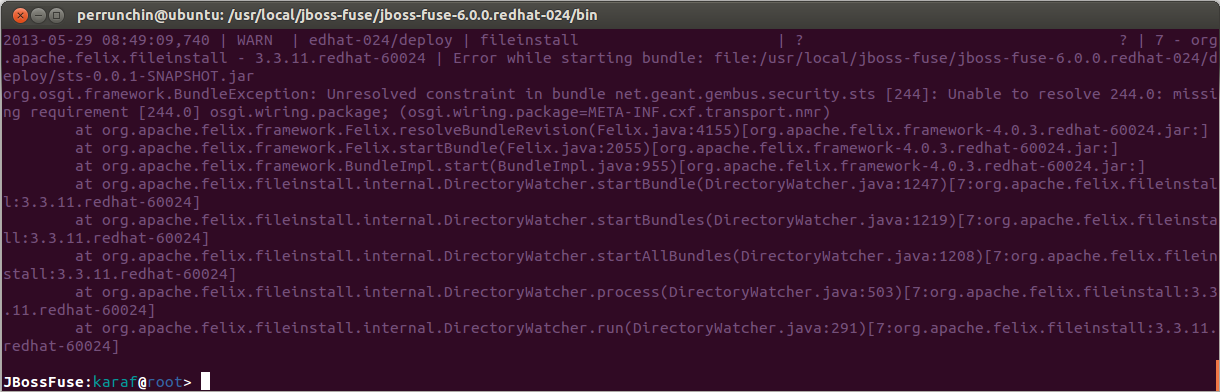
\includegraphics[width = 6.5 in]{Log_report}
			\end{figure}
		}
		
		\subsection{The Composition Service:}
		{
			Installing the composition service failed from the beginning given that both cookbook and Problems-with-cookbook state that it is necessary to run the command \textbf{features:install ode}. ODE is no longer supported and could not be installed.
		}
		
		\subsection{Epilogue:}
		{
			From that point on, I decided to move on to a different aspect of my research since getting GEMBus to work was really cumbersome and the only service that seems to be working properly is the registry service. \\
			
			When other aspects of my research are completed, I intended to go back and try to integrate my services with GEMBus to see if it is possible, or if more work from the GEMBus developers need to be done in order to correct the problems with the infrastructure.			
		}
	}
\end{document}